\section{Basics} \label{sec:basics}
The basic idea of \src{Core} is to have one object that controls the framework, one object for each floating panel and one object for each area where a floating panel can be docked.

\classbox{The controller is a \src{DockController}, the floating panels are \src{Dockable}s and the dock-areas are \src{DockStation}s.}

\subsection{Hello World}
Let's start with a simple hello world. This application uses the three basic components, the example consists of valid code and can run:
\begin{lstlisting}
import javax.swing.JFrame;

import bibliothek.gui.DockController;
import bibliothek.gui.dock.DefaultDockable;
import bibliothek.gui.dock.SplitDockStation;
import bibliothek.gui.dock.station.split.SplitDockGrid;

public class HelloWorld {
	public static void main( String[] args ) {
		DockController controller = new DockController();

		SplitDockStation station = new SplitDockStation();
		controller.add( station );
	
		SplitDockGrid grid = new SplitDockGrid();
		grid.addDockable( 0, 0, 2, 1, new DefaultDockable( "N" ) );
		grid.addDockable( 0, 1, 1, 1, new DefaultDockable( "SW" ) );
		grid.addDockable( 1, 1, 1, 1, new DefaultDockable( "SE" ) );
		station.dropTree( grid.toTree() );
	
		JFrame frame = new JFrame();
		frame.add( station.getComponent() );
	
		frame.setDefaultCloseOperation( JFrame.EXIT_ON_CLOSE );
		frame.setBounds( 20, 20, 400, 400 );
		frame.setVisible( true );
	}
}
\end{lstlisting}

\begin{figure}[h!]
  \centering
    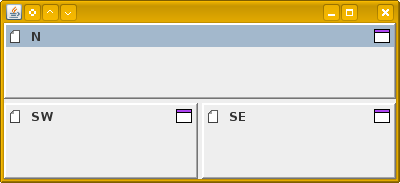
\includegraphics[width=0.5\textwidth]{basics/HelloWorld}
  \caption{The \src{HelloWorld} application.}
\end{figure}


What happens here? In line \src{10} a \src{DockController} is created. The controller will handle things like drag and drop. All elements will be in his realm. In line \src{12} a new \src{DockStation} is created and in line \src{13} this station is registered as root station at the \src{DockController}.

Then in line \src{15-19} a few children for \src{station} are generated. To set the layout of those children a \src{SplitDockGrid} is used. \src{SplitDockGrid} takes a few \src{Dockable}s and their position and puts this information into a form that can be understood by \src{SplitDockStation} (line \src{19}). It would be possible to add the \src{Dockable}s directly to the station, but this is the easy way.

In line \src{21} a new frame is created and in line \src{22} our \src{DockStation} is added to the frame.

\infobox{More demonstration applications can be found in the archive-file of \src{DockingFrames}. The demonstrations are stored in the project called ``tutorial``. You can use the ''tutorial.sh`` or ''tutorial.bat`` file to start them.}

\codebox{Another ''hello world`` can be found in the tutorial application under ''Basics/Core/Hello World``.}

\subsection{Dockable}
A \src{Dockable} represents a floating panel, it consists at least of some \src{JComponent} (the panel it represents), some \src{Icon} and some text for a title. Each \src{Dockable} can be dragged by the user and dropped over a \src{DockStation}.

Clients can implement the interface \src{Dockable}, but it is much less painful just to use \src{DefaultDockable}. A \src{DefaultDockable} behaves in many ways like the well known \src{JFrame}: title, icon and panel can be set and replaced at any time.

A small example:
\begin{lstlisting}
DefaultDockable dockable = new DefaultDockable();
dockable.setTitleText( "I'm a JTree" );
Container content = dockable.getContentPane();
content.setLayout( new GridLayout( 1, 1 ) );
content.add( new JScrollPane( new JTree() ) );
\end{lstlisting}

\warningbox{If implementing \src{Dockable}, pay special attention to the API-doc. Some methods have a rather special behavior. It might be a good idea to subclass \src{AbstractDockable} or to copy as much as possible from it.}

\designbox{A careful analysis of \src{Dockable} reveals that there is no way for applications to store their own properties within a \src{Dockable} (unless using a subclass...). There are two reasons for this.

First: if only using the default implementation, then clients do not have to worry about these properties. Storage of properties must and will be handled by the framework itself.

Second: Components of the framework cannot get any unfair advantage over custom components. Everything has to be designed in a way that it can work with new and unexpected implementations of \src{Dockable}.}

\subsection{DockStation}
\src{Dockable}s can never fly around for themselves, they need a \src{DockStation} as anchor point. The relationship between \src{DockStation} and \src{Dockable} can best be described as parent-child-relationship. A \src{DockStation} can have many children, but a \src{Dockable} only one parent.

There are some classes which are \src{DockStation} and \src{Dockable} at the same time. They allow to build a tree of \src{DockStation}s and \src{Dockable}s. A controller can handle more than just one tree and \src{Dockable}s can switch from one tree to another.

Clients can implement new \src{DockStation}s. But be warned that the interface contains many methods and a lot of them require a lot of code. Don't expect to write less than 1000 lines of code.

A small example that builds a \src{StackDockStation}:
\begin{lstlisting}
StackDockStation stack = new StackDockStation();
stack.setTitleText( "Stack" );
stack.drop( new DefaultDockable( "One" ) );
stack.drop( new DefaultDockable( "Two" ) );
\end{lstlisting}
Some observations: \src{StackDockStation} is a \src{Dockable} as well, in line \src{2} the title is set. Two \src{DefaultDockable}s are put onto the station in lines \src{3,4}, the method \src{drop} is available in all \src{DockStation}s.

\warningbox{\src{DockStation}s are the most complex classes within the framework, they are also among the most important classes. It is very uncommon to subclass them or to write new ones. If you think you need to subclass a \src{DockStation}, be sure to have explored all other options.}

\src{Core} offers a collection four different stations. These are listed in the remainder of this section. Additional details can be found in chapter \ref{sec:stations}.

\subsubsection{StackDockStation}
This station is organized like a \src{JTabbedPane}. Only one child is visible, but another can be made visible by clicking some button. The framework will automatically create new \src{StackDockStation}s when a \src{Dockable} is dragged over another. Also \src{StackDockStation}s with only one child get automatically replaced by this child.

\begin{figure}[h!]
  \centering
    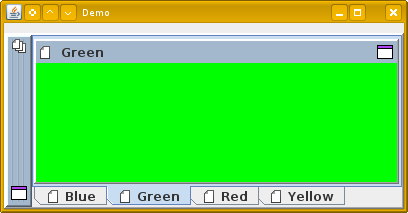
\includegraphics[width=0.5\textwidth]{basics/StackDockStation}
  \caption{A \src{StackDockStation} with four children on a frame.}
\end{figure}

\classbox{
The station consists of four layers, as seen in the image below. There is a background panel (1) which just is some \src{Container} to put other things onto it. Then there is a selection layer (2), which is represented by an instance of \src{StackDockComponent}. Above that is a \src{DockableDisplayer} (3) for each \src{Dockable}. The displayers paint some decorations that depend on the \src{Dockables} in the topmost layer (4).

\hspace{0.20\textwidth} 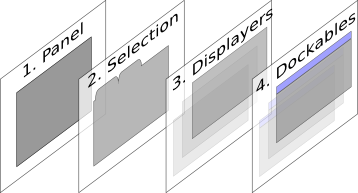
\includegraphics[width=0.75\textwidth]{basics/stack}
}

\subsubsection{SplitDockStation}
All the children of this station are visible. The user controls the children as if the station would consist of many \src{JSplitPane}s set into each other (hence the name). Internally the station is organized as tree, where a leaf is a \src{Dockable} and a node the gap between two sets of \src{Dockable}s. Furthermore this station offers a ``fullscreen mode'' where one of its children takes up the entire space and all other children are invisible.

\begin{figure}[h!]
  \centering
    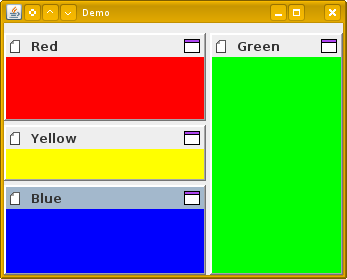
\includegraphics[width=0.5\textwidth]{basics/SplitDockStation}
  \caption{A \src{SplitDockStation} with four children on a frame.}
\end{figure}

\classbox{
Like the \src{StackDockStation}, this station consists of four layers. Layers 1, 3 and 4 are identical to the layers of the \src{StackDockStation}. A background panel (1), \src{DockableDisplayers} (3) to paint decorations and the children (4). Layer 2 is the logical tree which tells how to lay out the children. The nodes of this tree consist of \src{SplitNode}s and the root can be accessed through the method \src{getRoot}. Clients should never add or remove nodes from the tree directly.

\hspace{0.20\textwidth} 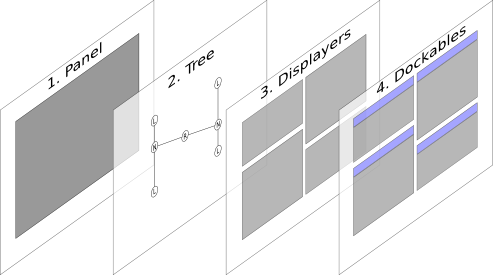
\includegraphics[width=0.75\textwidth]{basics/split}
}

\subsubsection{FlapDockStation}
This station is a list of buttons. If the user clicks on one of the buttons a window opens showing a child. Only one child can be shown at a time. This station can be used as sidebar to collect ``minimized'' \src{Dockables}. 

\begin{figure}[h!]
  \centering
    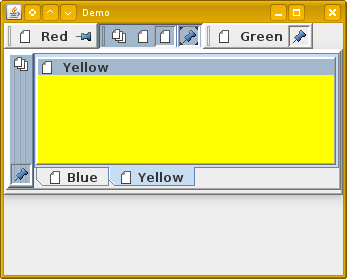
\includegraphics[width=0.5\textwidth]{basics/FlapDockStation}
  \caption{A \src{FlapDockStation} with three children on a frame. The selected child is a \src{StackDockStation} containing two more children.}
\end{figure}

\classbox{
\src{FlapDockStation} consists of 5 layers. A background panel (1) as \src{Container} for other components. A set of buttons (2), each button is a \src{DockTitle}. Then there is the window that shows the current selection (3), an instance of \src{FlapWindow}. A displayer (4) to paint decorations and the \src{Dockable} child (5) that is selected.

\hspace{0.20\textwidth} 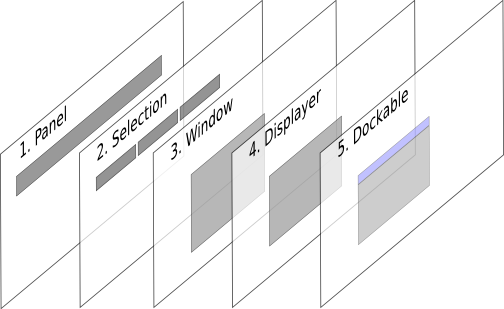
\includegraphics[width=0.75\textwidth]{basics/flap}
}

\subsubsection{ScreenDockStation}
The \src{ScreenDockStation} allows its children to float around freely on the screen. Each child is put onto its own window which is independent from any other window. This station also offers a ``fullscreen mode'' where a window is enlarged to fill the entire space of a screen.

\begin{figure}[h!]
  \centering
    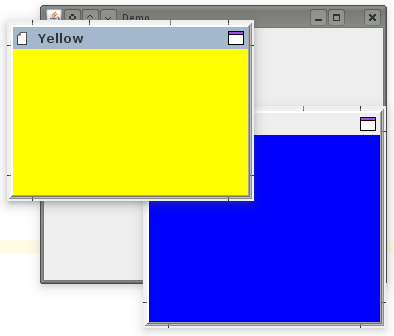
\includegraphics[width=0.5\textwidth]{basics/ScreenDockStation}
  \caption{A \src{ScreenDockStation} with two children floating over a frame.}
\end{figure}

\classbox{
This station is pretty simple and consists of only 3 layers. Some windows (1), instances of \src{ScreenDockWindow}, provide a container to show the children. On each window there is a \src{DockableDisplayer} (2) to paint decorations, and on top is one \src{Dockable} child (3).

\hspace{0.20\textwidth} 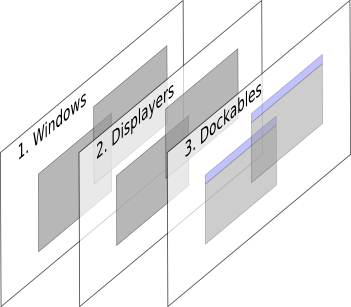
\includegraphics[width=0.75\textwidth]{basics/screen}
}

\subsection{DockController}
A \src{DockController} holds \src{Dockable}s, \src{DockStation}s and other supporting elements together. Most tasks are not handled by the \src{DockController} but by one of its sub-controllers, e.g. drag and drop is handled by the \src{DockRelocator}.

There can be more than one \src{DockController} in an application. Each controller has its own realm and there is no interaction between controllers. But most applications will need only one \src{DockController}.

Clients need to register the roots of their \src{DockStation}-\src{Dockable}-trees. \linebreak They can use the method \src{add} of \src{DockController} to do that. All children of the root will automatically be registered as well. If a \src{DockStation} is not registered anywhere, it just does not work properly. For \src{Dockable}s one could say that registration equals visibility. A registered \src{Dockable} can be seen by the user, an unregistered not.

\classbox{\src{DockController} uses other classes to handle tasks. Many of these classes can be observed by listeners. An incomplete list:

\src{DockRegister}: a list of all \src{Dockable}s and \src{DockStation}s.

\src{DockRelocator}: handles drag and drop operations, can create a \src{Remote} to play around without user interaction.

\src{DoubleClickController}: detects double clicks on \src{Dockable}s or on components which represent \src{Dockable}s.

\src{KeyBoardController}: detects \src{KeyEvent}s on \src{Dockable}s or on components which represent \src{Dockable}s.}

\warningbox{Never forget to register the root-\src{DockStation}(s) at the \src{DockController} using the method \src{add}.}

\designbox{Why not just one \src{DockController} implemented as singleton? A singleton would make many interfaces simpler, eliminating all the code where the controller is handed over to even the smallest object. But there is absolutely no reason why only one controller should exist. A controller has no unique property that would justify a singleton. And not using a singleton gives more flexibility.}

\subsection{DockFrontend}
\src{DockController} only implements the basic functionallity. While this allows developers to add new exciting shiny customized features, it certainly doesn't help those developers which just want to use the framework.

The class \src{DockFrontend} represents a layer before \src{DockController} and adds a set of helpful methods. Especially a ``close''-button and the ability to store and load the layout are a great help. \src{DockFrontend} replaces \src{DockController}, clients should add the root-\src{DockStation}s directly to the frontend, not to the controller. They can use the method \src{addRoot} to do so.

\warningbox{\src{DockFrontend} adds a few nice features but not enough to write an application without even bothering to have a look at \src{DockingFrames}. Developers which can live with not having absolute control over the framework should use \src{Common}. \src{Common} adds all those features which make a docking-framework complete, e.g. a ``minimize''-button}

\designbox{\src{DockFrontend} was written long after \src{DockController}. For the most part it just reuses code that already exists. It would be possible to write two applications with exact the same behavior once with and once without \src{DockFrontend}. The only thing that \src{DockFrontend} adds to the framework is a central hub where all the important features are accessible and a good set of default-values for various properties of the framework.}

\infobox{Use the methods called \src{setDefault...} to set default values for properties which will be used for all \src{Dockable}s, e.g. whether \src{Dockable}s are hideable or not.}

\subsubsection{Close-Button}
In order to show the close-button clients need first to register their \src{Dockable}s. The method \src{addDockable} is used for that. Each \src{Dockable} needs a unique identifier that is used internally by \src{DockFrontend}. Later clients can call the method \src{setHideable} to show or to hide the close-button.

By calling the method \src{setShowHideAction} clients can make the buttons invisible for all \src{Dockable}s, note however that the \src{Dockable}s hideable-property is not affected by this method.

If clients want to control whether a \src{Dockable} can be closed, they should add a \src{VetoableDockFrontendListener} to the \src{DockFrontend}. This listener will be informed before a \src{Dockable} is made invisible and allows to cancel the operation.

\designbox{Why is the close-button not part of the very core of the framework? For one because the very core works on abstract levels and should not be made more complex with special cases like this button. There are also different implementations of this button and not all perform the same actions when pressed (this is especially true when using \src{Common}).}

\subsubsection{Storing the layout}
The methods \src{save}, \src{load}, \src{delete} and \src{getSettings} are an easy way to store and load the layout. This mechanism will be explained in detail in another chapter.